\chapter{CONCLUSION AND FUTURE RECOMMENDATION}
\section{Lesson Learnt/Outcome}
\subsection{Home Page}
At the top of the home page, there's a header section that includes the project logo, navigation menu, and user login/signup options. This section provides easy access to different parts of the platform and allows users to log in or create an account.
\begin{figure}[H]
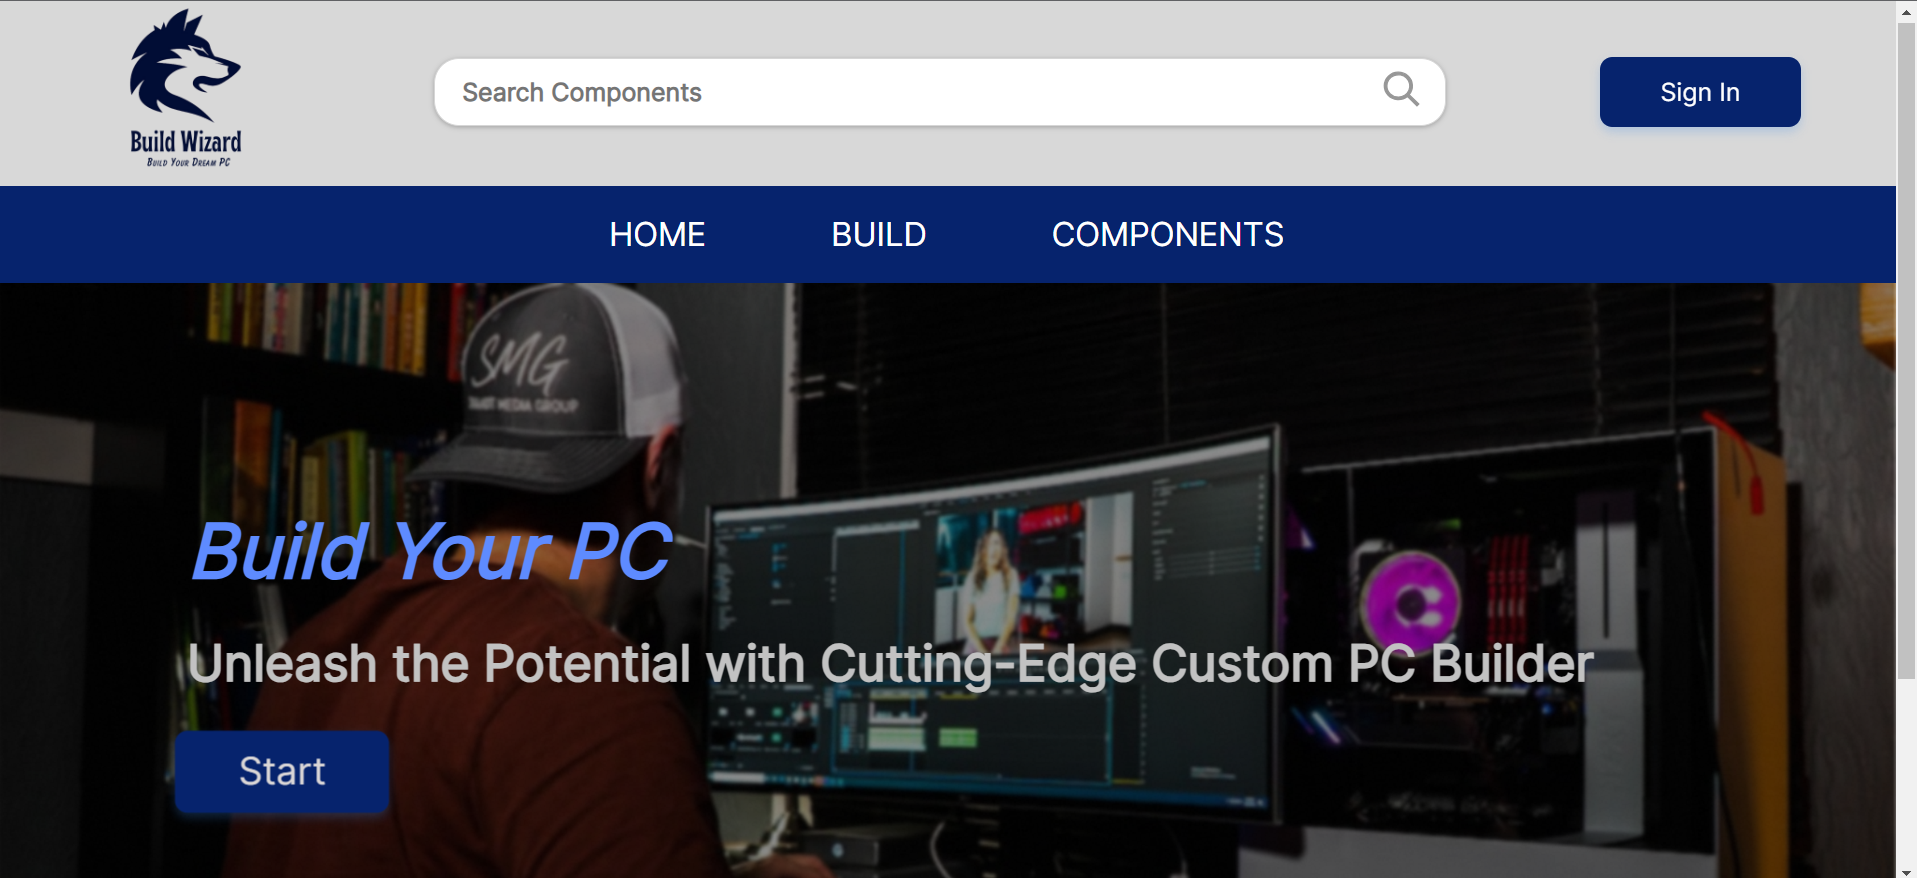
\includegraphics[width=15cm]{Diagrams/UIHOME.png}
\caption{Home Page}
\end{figure}
\newpage
\subsection{Build Page}
A Build Page within the context of the Build Wizard :PC part picker project refers to a dedicated section of the platform where users can create and customize their own PC configurations. This page allows users to select various computer components, such as processors, graphics cards, memory modules, storage devices, and more, to assemble a complete and functional computer system tailored to their specific needs and preferences.
\begin{figure}[H]
\centering
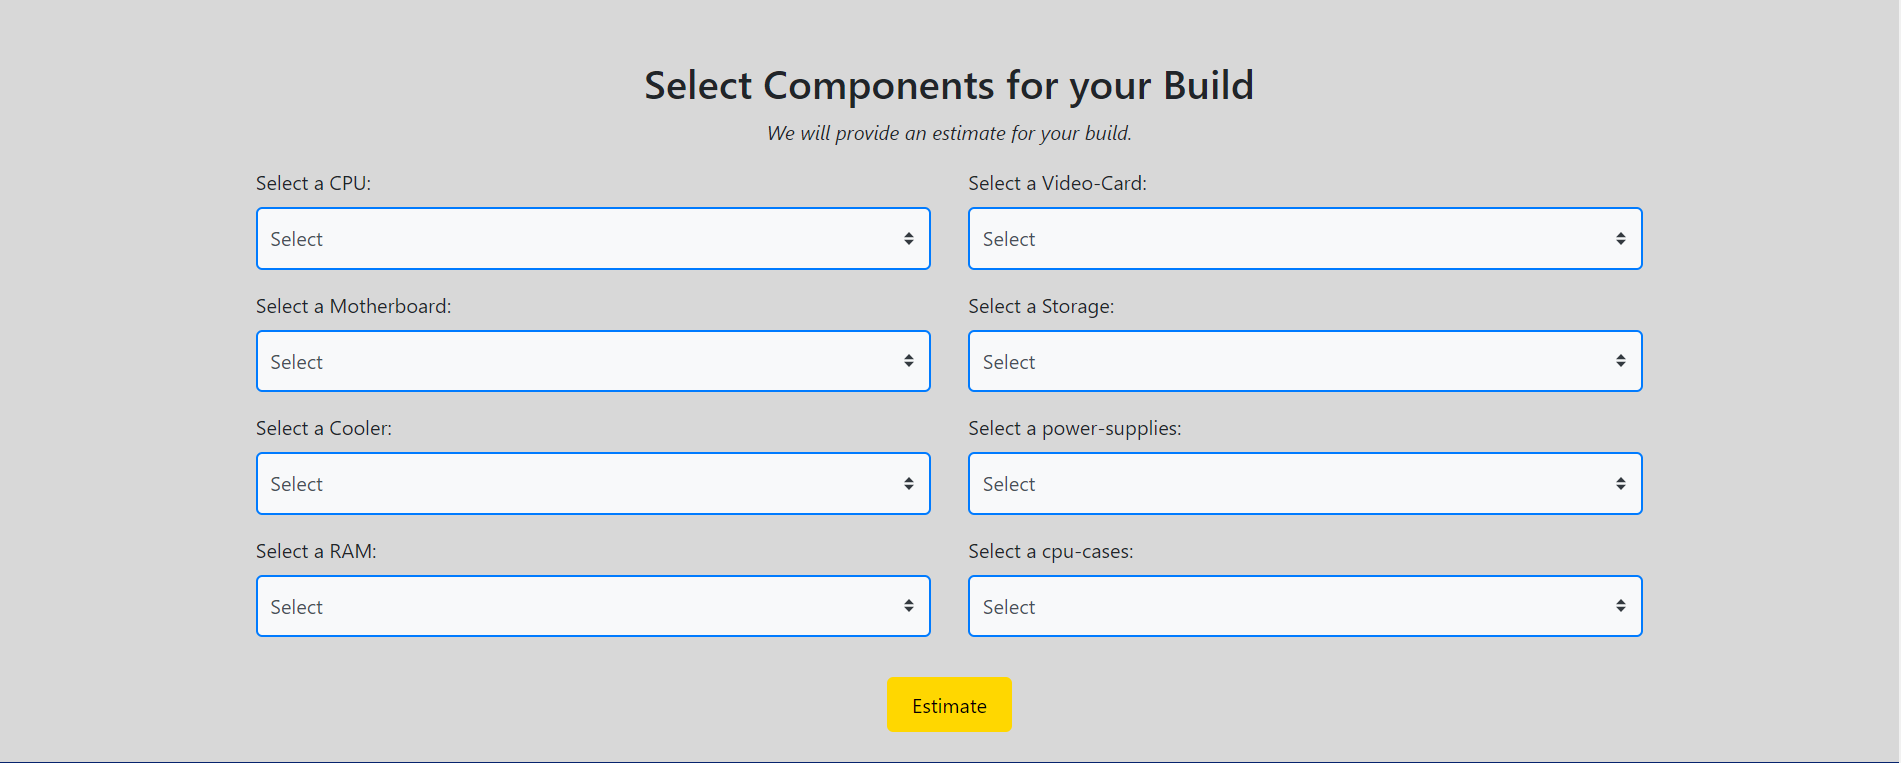
\includegraphics[width=16cm]{Diagrams/newbuildpage.png}
\caption{Build Page}
\end{figure}
\subsection{Components Page}
The "Components" page for this project, focusing on building a user-friendly platform for veiwing pc components and their information. It's crucial to design this page to be intuitive, informative, and visually appealing to provide a better experience.
\begin{figure}[H]
    \centering
    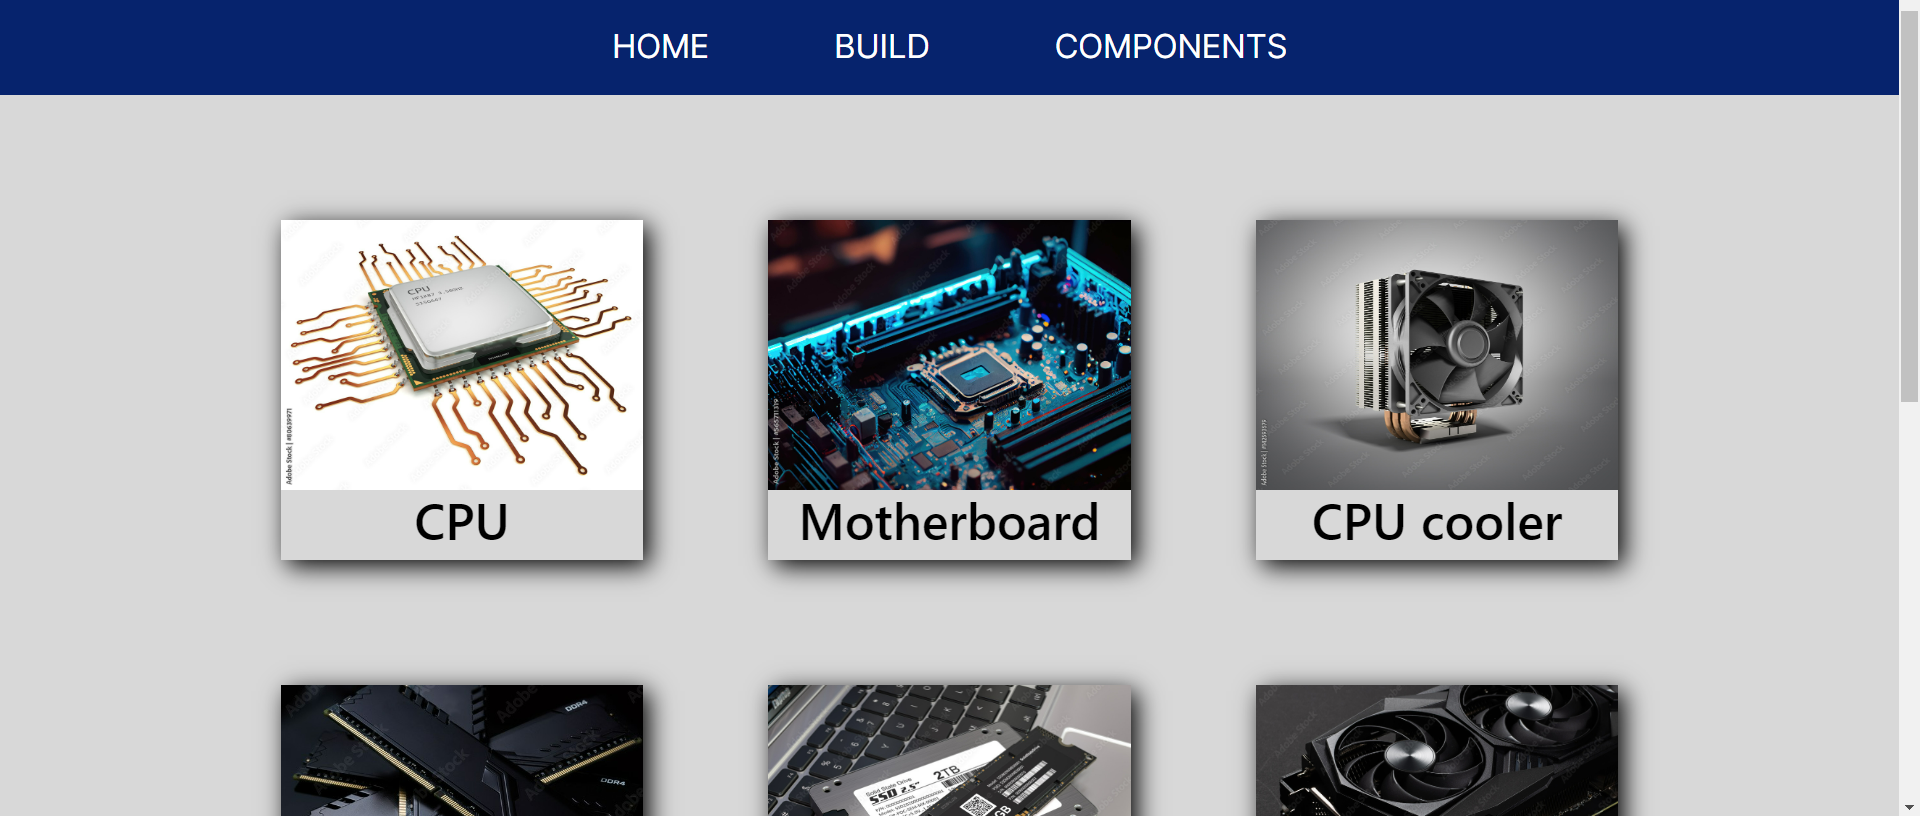
\includegraphics[width=16cm]{Diagrams/components.png}
    \caption{component Page}
    \end{figure}
\subsection{Admin Portal}
The admin portal for this project serves as a centralized interface accessible to authorized administrators, allowing them to manage componets for the webpage.
\begin{figure}[H]
    \centering
    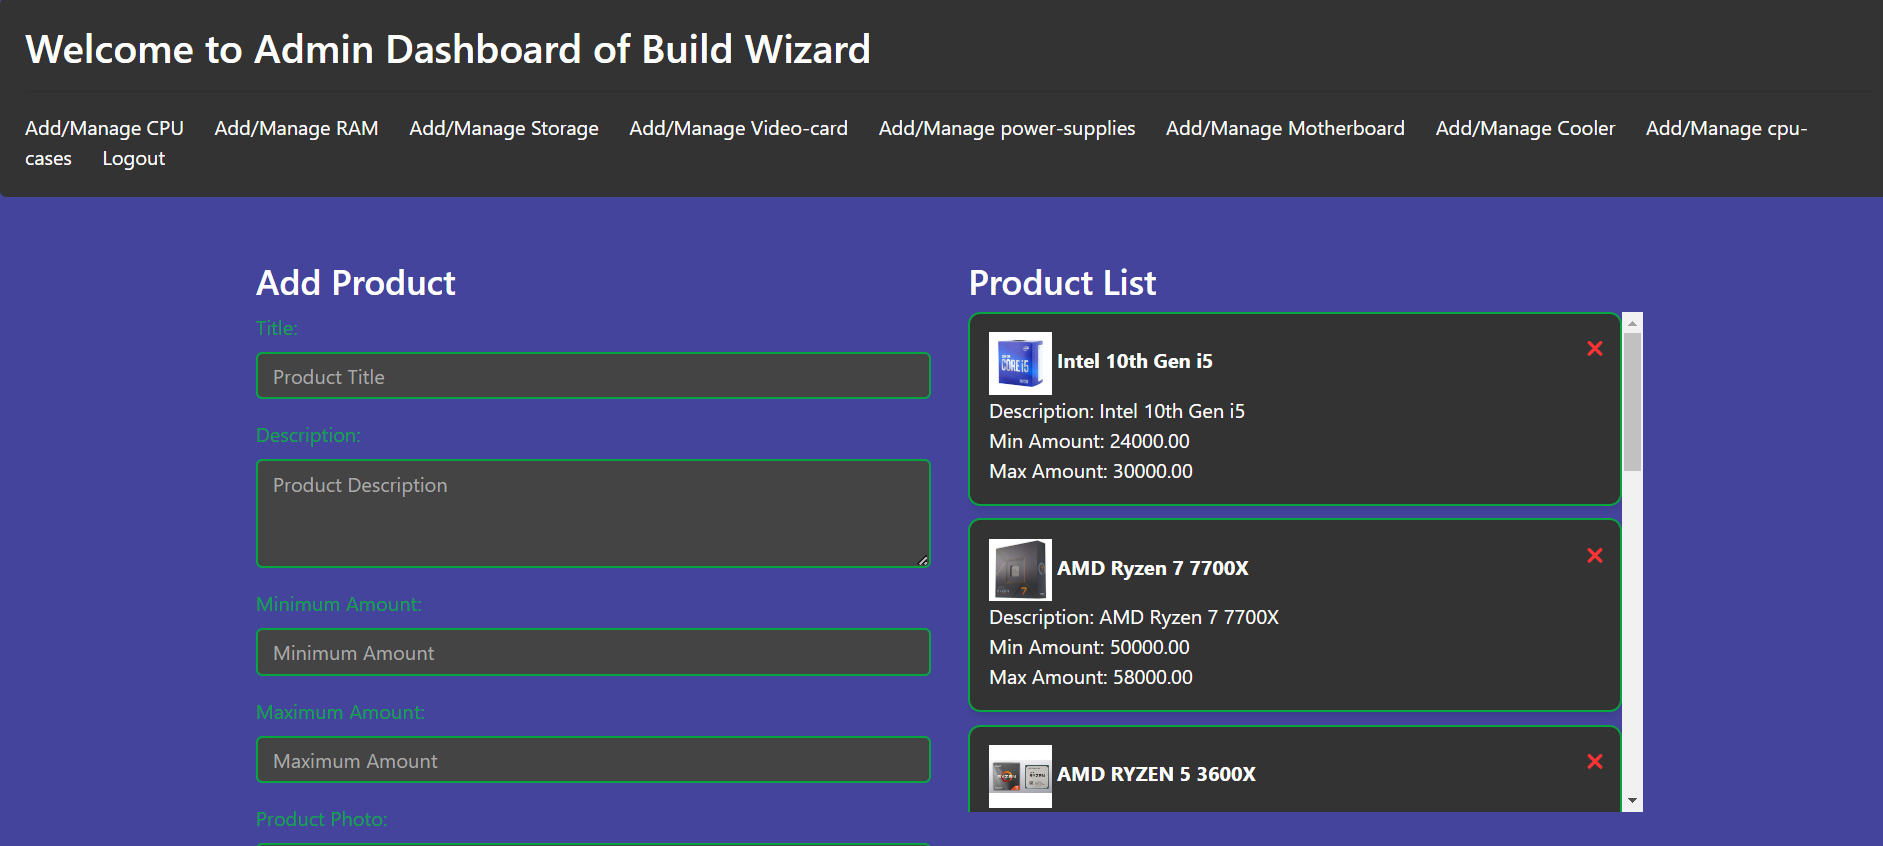
\includegraphics[width=16cm]{Diagrams/admin_portal.png}
    \caption{Admin Page}
    \end{figure}
\subsection{Sign-in Page}
\begin{figure}[H]
    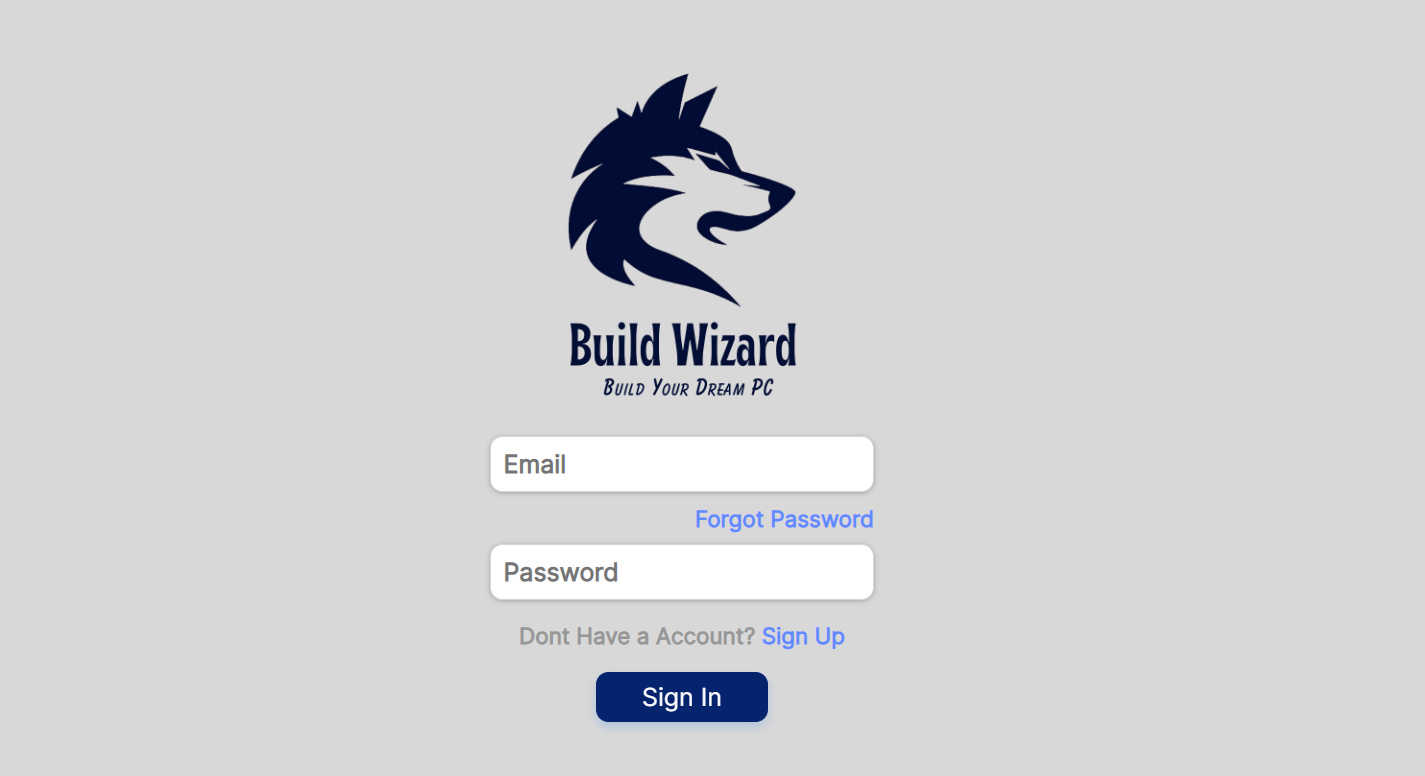
\includegraphics[width=16cm]{Diagrams/UILOGIN.png}
    \caption{SignIn Page}
    \end{figure}
    \subsection{Incorrect Password}
    \begin{figure}[H]
        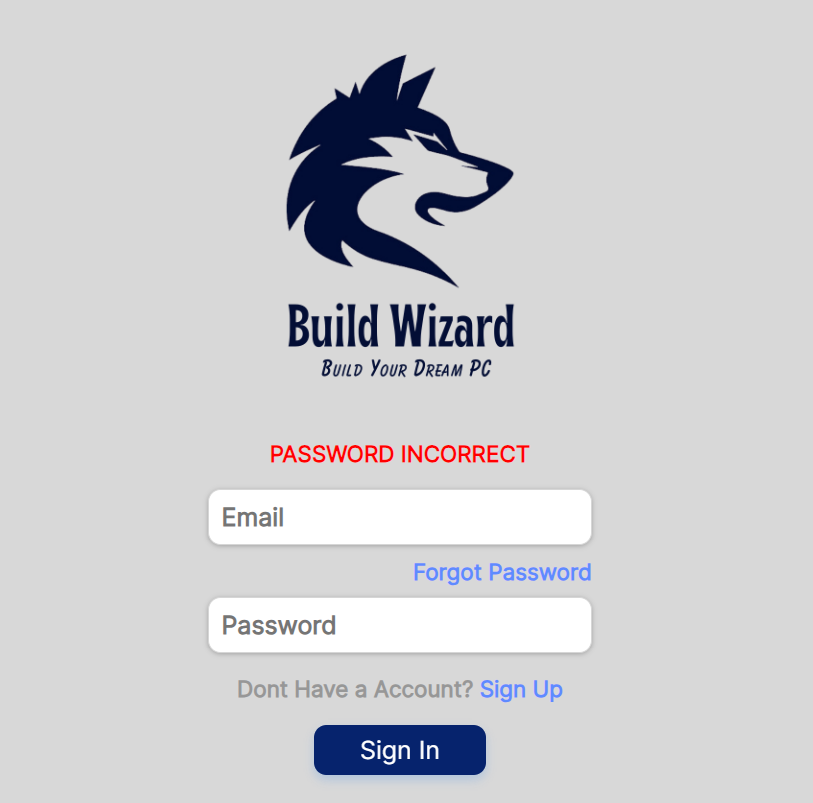
\includegraphics[width=15cm]{Diagrams/incorrect password.png}
        \caption{Incorrect Password}
        \end{figure}
\subsection{Sign-up Page}
\begin{figure}[H]
    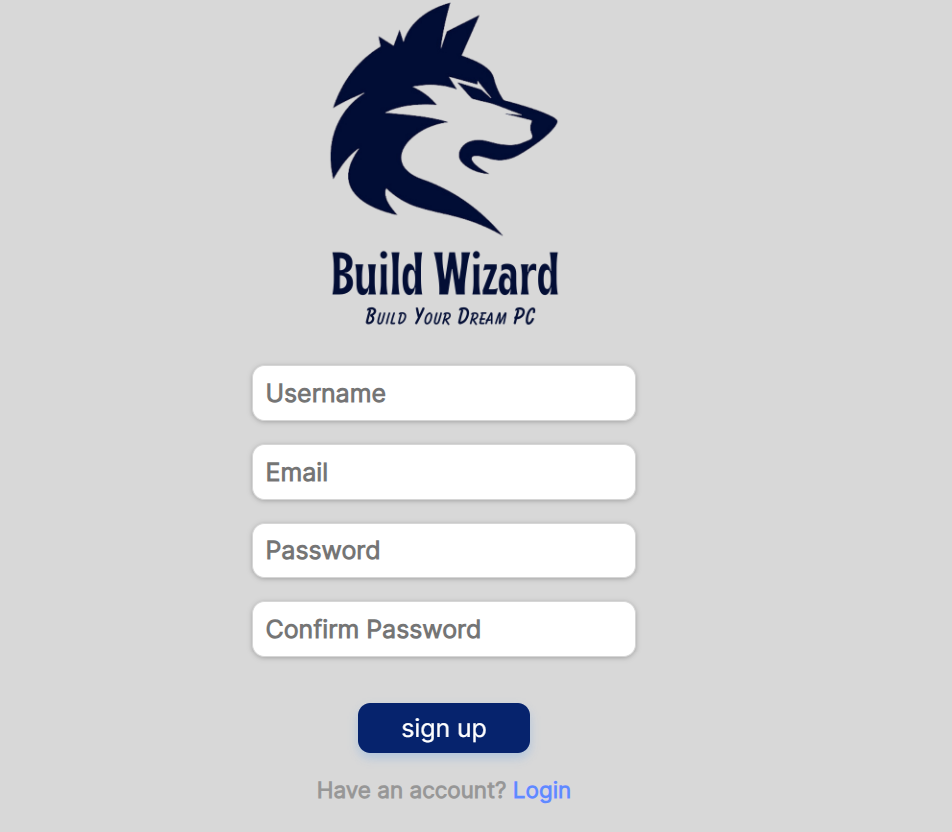
\includegraphics[width=16cm]{Diagrams/UISIGNUP.png}
    \caption{SignUp Page}
    \end{figure}
    \subsection{Searching Page}
\begin{figure}[H]
    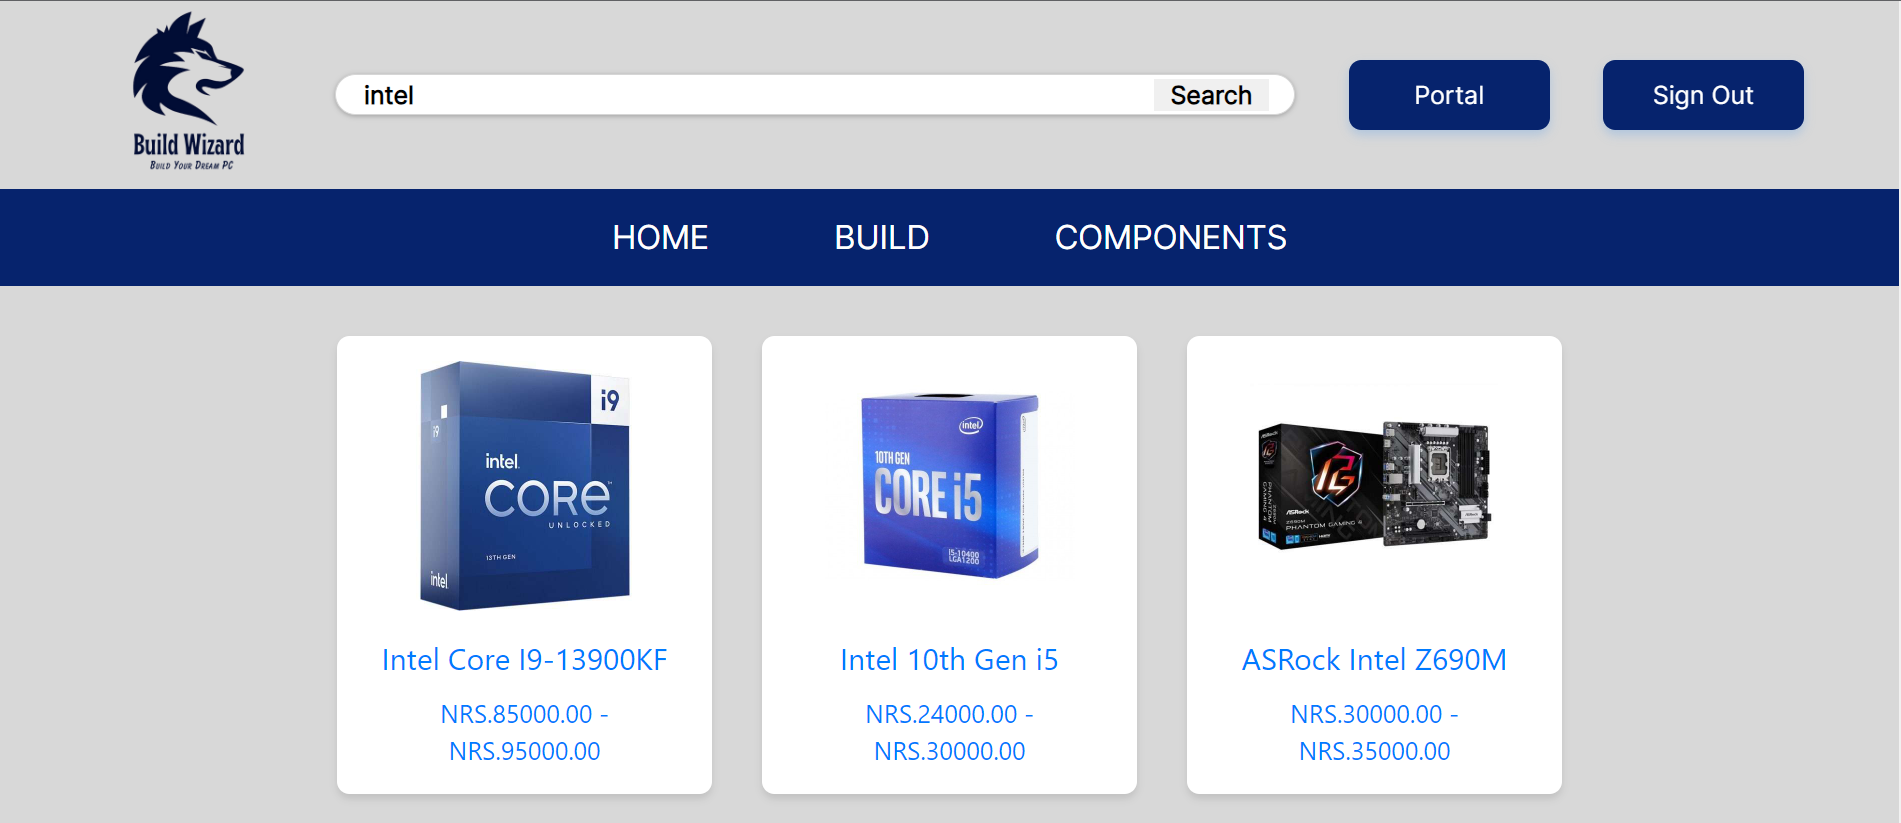
\includegraphics[width=16cm]{Diagrams/searching.png}
    \caption{Searching Page}
    \end{figure}
\section{Conclusion}
In conclusion, the Build Wizard project is an innovative online platform tailored for the Nepalese PC building community. It addresses compatibility challenges and facilitates price comparisons. This localized solution simplifies the PC building process, promoting informed decisions and enhancing the overall PC building experience in Nepal.
\section{Future Recommendations}
\begin{itemize}
    \item \textbf{Vendors:} In future ,Local vendors can feature products.
    \item \textbf{Ordering System:} Odering and delivary system can be integrated.
    \item \textbf{Mobile Accessibility:} System will accessible and user-friendly on mobile devices, as many users may prefer to use it on smartphones or tablets.
    \item \textbf{Offline Customization:} This would allow users to customize the system and use it even when they don't have an internet connection. This can be particularly useful in situations where a stable internet connection is not guaranteed.
\end{itemize}